\chapter{Distribution Networks for Scalable P\&R}\label{chapter:Methodology}
This chapter proposes three different signal Distribution Networks (DNs) that overcome the restrictions of the placement and routing algorithm, ortho, which was reviewed as the state of the art in Chapter~\ref{chapter:SotA}. One restriction of ortho is the big area usage and the high number of wire crossings. To reduce these shortcomings an Ordering DN (ODN) is proposed in this thesis. The second big restriction ortho has, is that majority functions need to be decomposed into multiple gates, even though QCA technology provides a majority gate. In this thesis a Majority Gates DN (MGDN) is introduced, which enables ortho to make use of this theoretical advantage. Also ortho is not able to place any sequential circuits. Therefore, a Sequential DN (SDN) is introduced.

The placement and routing algorithm, ortho, has been shown to have limitations regarding area usage, wire crossings, majority gates and sequentiality, but it still possesses a powerful placement and routing procedure. To overcome these limitations, it is proposed to maintain the foundation of the algorithm while incorporating new functionalities. The functionalities include an ordering of inputs and the placement and routing of majority gates and sequential QCA circuits. However, these new functionalities often result in irregularities, such as in the clocking or routing, and the goal of the proposed signal DNs is to redistribute signals on the layout in a way that these irregular parts align with the regular placement and routing while still satisfying all design constraints. In this way, the algorithm can still function in a similar manner as ortho. However, the underlying logic network and the placement and routing must also be modified to incorporate the desired functionalities, adding complexity to the preprocessing and algorithm.

Since ortho is restricted to the use of only 2DD-Wave clocking, the signal DNs must have the ability to change the clocking in the layout to implement their respective functionalities, regarding the implementation of majority gates and sequentiality. Therefore, the implementation of these networks must be done with care and synchronization constraints must be closely considered.

The ODN is discussed first, which aims to reduce the area in the input region of the layout. Afterwards, the networks used for implementing majority gates and sequential parts are discussed and analyzed.

\section{Ordering Distribution Network (ODN)}

\begin{figure}
	\centering
	\subfigure[Placement and routing of a 2:1 MUX network using the ortho algorithm]
	{
		\centering
		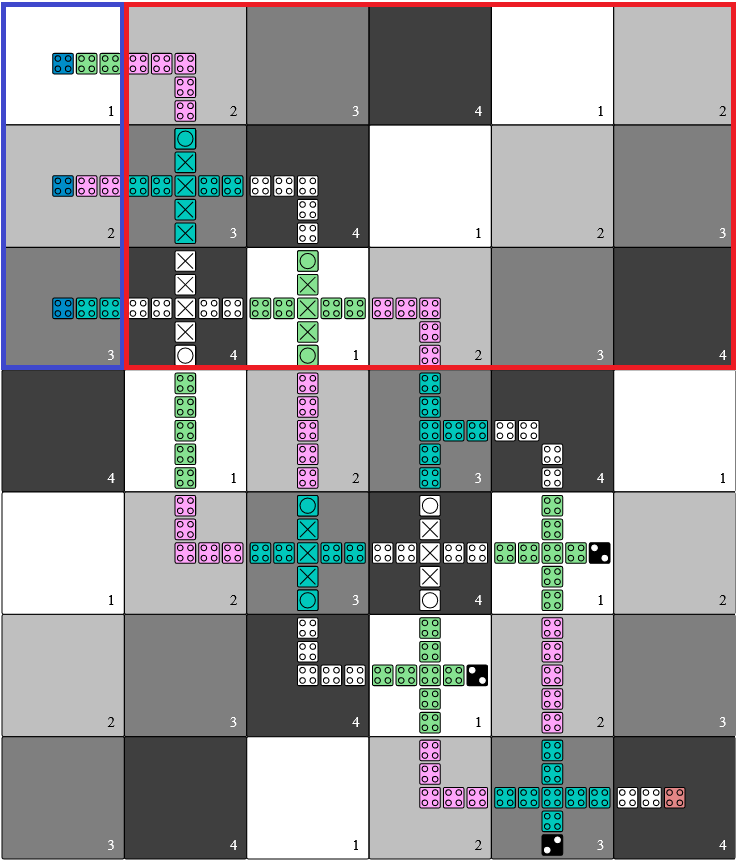
\includegraphics[scale=0.4]{ortho_mux_21_marked}
		\label{subfig:ortho_mux_21}
	}
	\subfigure[Placement and routing of a 2:1 MUX network using the ortho algorithm with the ODN]
	{
		\centering
		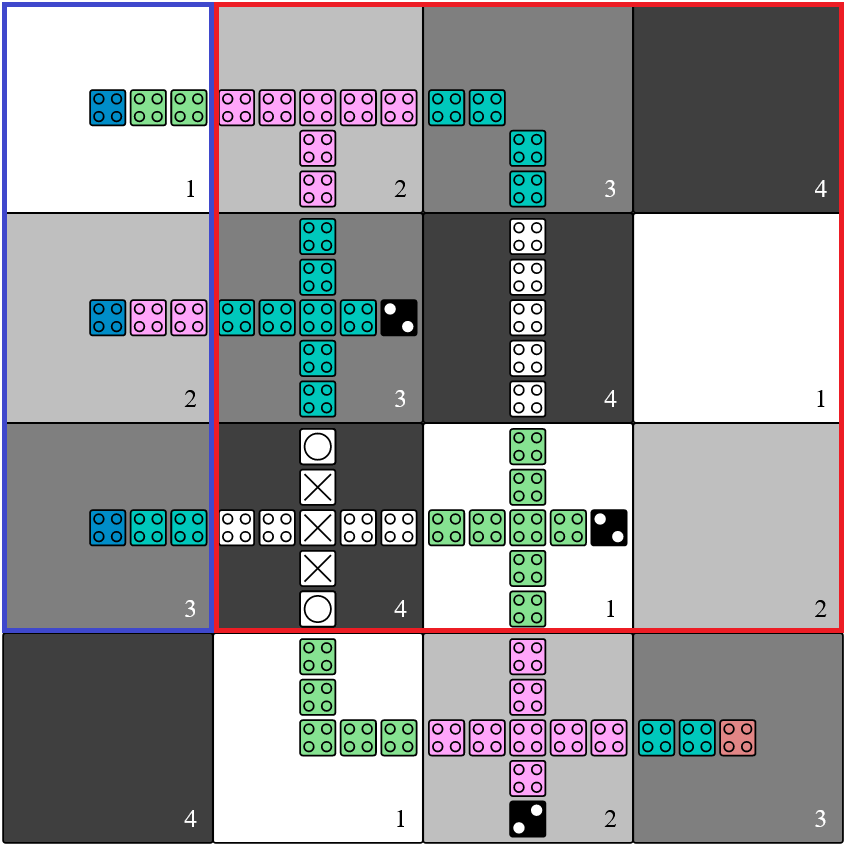
\includegraphics[scale=0.346]{input_network_mux_21_marked}
		\label{subfig:input_network_mux_21}
	}
	\caption{Comparison of ortho and ortho including ODN}\label{fig:input_network_mux_21}
\end{figure}


In this section, we propose the use of an Orthogonal Data Network (ODN) within ortho for the scalable placement and routing of QCA circuits. The goal of the ODN is to minimize wire crossings and maximize use of space by ordering and placing inputs in a specific way. As shown in Figure~\ref{fig:input_network_mux_21}, the ODN significantly reduces area usage and the number of wire crossings when compared to a traditional orthogonal design. This is achieved through two main concepts: (1) reordering of primary inputs and (2) utilizing the input area for gate placement. In Figure~\ref{subfig:ortho_mux_21} and Figure~\ref{subfig:input_network_mux_21} the PIs and the repective reordered PIs are marked blue and the input area is highlighted red. These concepts are further explained in detail in the following sections, and the implementation of the ODN requires four steps to be integrated into the orthogonal algorithm. These include the ordering of primary inputs, the implementation of conditional coloring, the introduction of a new rule for placement and routing, and the application of inverter balancing.

\subsection{Ordering of PIs}

In this section, we discuss the ordering of PIs in our design. Considering an AND-gate connecting two inputs, it is ideal for the two PIs to be placed directly under each other in order to reduce the amount of wiring needed. When the two PIs are placed, for instance, in the first and last row of a layout, the distance that must be covered is greater and the probability of wire crossings increases. This highlights the importance of proper PI ordering in reducing wiring and minimizing wire crossings.

\begin{figure}
	\centering
	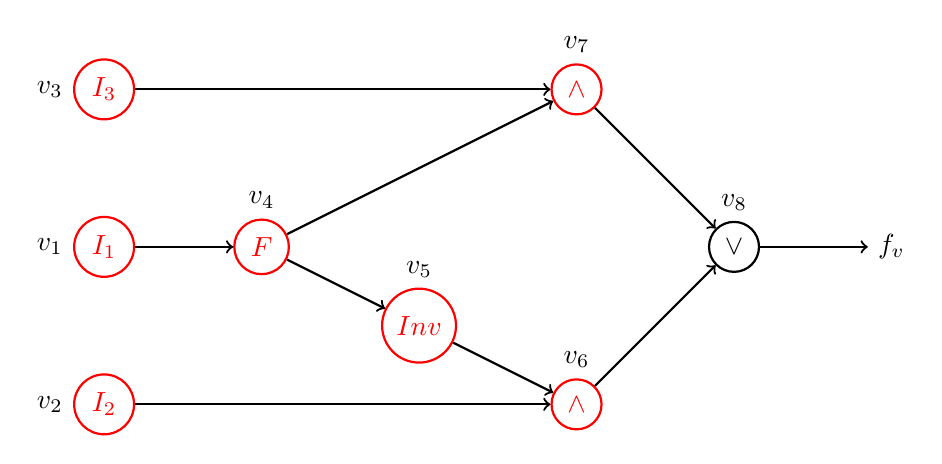
\begin{tikzpicture}[node distance={2cm and 2cm}, thick, scale=1, main/.style = {draw, circle}] 
		\node[main, color=red] (3) at (0,0) [label=west:$v_3$]{$I_3$}; 
		\node[main, color=red] (1) at (0,-2)[label=west:$v_1$] {$I_1$};
		\node[main, color=red] (2) at (0,-4)[label=west:$v_2$] {$I_2$};
		
		\node[main, color=red] (4) at (2,-2)[label=north:$v_4$]{$F$}; 
		
		\node[main, color=red] (5) at (4,-3)[label=north:$v_5$]{$Inv$};
		\node[main, color=red] (6) at (6,-4)[label=north:$v_6$]{$\wedge$};
		\node[main, color=red] (7) at (6,0)[label=north:$v_7$]{$\wedge$};
		
		\node[main] (8) at (8,-2)[label=north:$v_8$]{$\vee$};
		
		\node (f) at (10,-2) {$f_v$};
		
		
		\draw[->, above] (1) -- (4);
		\draw[->, above] (2) -- (6);
		\draw[->, above] (3) -- (7);
		\draw[->, above] (5) -- (6);
		\draw[->, above] (4) -- (5);
		\draw[->, above] (4) -- (7);
		\draw[->, above] (6) -- (8);
		\draw[->, above] (7) -- (8);
		\draw[->, above] (8) -- (f);
		
		
	\end{tikzpicture}
	\caption{Logic Network of a 2:1 MUX with gates viewed in the ODN}\label{fig:mux_LN_in}
\end{figure}

\begin{figure}
	\centering
	\begin{tikzpicture}[node distance={2cm and 2cm}, thick, main/.style = {draw, rectangle}] 
		\node[fit={(0,0) (8, 8)}, inner sep=0pt, draw=black, thick] (frame) {};
		\node[fit={(1.5,0) (6.5, 8)}, inner sep=0pt, draw=black, thick, fill=cyan] (logic) {Combinational logic};
		\node[fit={(0,6.5) (1.5, 8)}, inner sep=0pt, draw=black, thick, fill=TUMGray] (PIs) {ordered \\ PIs};
		\node[fit={(6.5,0) (8, 8)}, inner sep=0pt, draw=black, thick, fill=TUMGray] (POs) {POs};
		
		\draw[] (1, 6.5) -- (6.5, 6.5);
		
		\draw (4,7.25) node [align=left] {Gates viewed \\ in the ODN};
		
		
	\end{tikzpicture} 
	\caption{Scheme of area usage in the layout using the ODN} \label{fig:ordering_scheme}
\end{figure}

To examine the concept, it is necessary to first identify the part of the logic network that is considered for the ODN. This can be determined by examining the nodes that are placed in the input area. These include nodes that are directly connected to the PIs and nodes that are connected to these nodes and colored east. For the network, all nodes that are successively connected, starting at each PI and ending at the first node with two fan-ins, are considered. Figure~\ref{fig:mux_LN_in} shows this principle. Once these nodes are placed correctly, all conflicts are resolved, and the ortho algorithm can function as intended. The schmetic of a resulting ayout is depicted in Figure~\ref{fig:ordering_scheme}.

For the ordering, PIs connected to the same two-fanin gate are placed consecutively, first placing PIs connected to fan-outs and minimizing the routing distance thus reducing the probability of wire crossings. Figure~\ref{fig:mux_LN_in} shows that all three PIs are connected over the two AND-gates. First the PI connected to the fan-out is placed. Second the PI with the branch without an inverter is placed and then the PI with the inverter in its branch.

Additionally, after reordering the PIs, the remaining logic network is ordered topologically, so that the improvements following the ordering of the PIs can be applied to the entire network. In the following the steps allowing the use of the input area are proposed. Therefore, first the conditional coloring and then a new P\&R rule are discussed.

\subsection{Conditional Coloring}

In this section a conditional coloring is proposed, which finds a valid coloring for the gates viewed by the ODN and allows a placement and routing of these gates without resulting in conflicts. Recalling the pseudo-code from the ortho Algorithm~\ref{alg:ortho}, an input has a conflict when the gate connected to it is colored $south$, which would lead the routing to wire over the other inputs in the same column, which is not allowed. This means that the area overhead in the input region is highly dependent on the coloring assigned to the outgoing edges of the inputs. Line $3$ of the pseudocode of ortho, which invokes the coloring algorithm, finds a valid but not an optimal coloring for the given logic network. Unfortunately, due to the algorithm's nature, it often assigns the color $south$ to edges connected to PIs resulting in conflicts and area overhead.

In the following, the conditional coloring is discussed regarding different gate-types, which can be connected to PIs. Figure~\ref{fig:mux_LN_clr} shows the conditional coloring chosen for the logic network of a 2:1 MUX. It has to be noted, that the chosen coloring already considers the new rule for PIs with edges connected to gates colored south.
The direction assignment for one-fanin nodes, including inverters and fan-out nodes, can be chosen arbitrarily as the PI to which they are connected has only one outgoing edge, resulting in no dependencies. In this case, the non-conflicting $east$ assignment can always be chosen. When examining two-input logic gates such as AND and OR gates, the coloring can only be chosen arbitrarily if both incoming nodes are PIs, again allowing for the non-conflicting assignment of east. In all other cases, the direction assignment must consider the coloring of the other incoming edge of the gate. To determine dependencies, all one-fanin nodes must first be colored, including inverters and fan-outs.

Regarding fan-outs, following the coloring rules, the two outgoing edges need to be colored in different directions, so that the fan-out gates placed into the network have one output assigned with color $east$ and one output assigned with color $south$. Considering that the second coloring constraint requires both incoming edges of the gate connected to the edge colored $south$, also to be colored $south$, and the second incoming edge being connected to a PI, we again get a conflict and we can see that a conditional coloring alone is not powerful enough to resolve all conflicts.

To enable the use of the input area, additionally a new rule for edges colored $south$ is introduced, making the rewiring redundant.

\begin{figure}
	\centering
	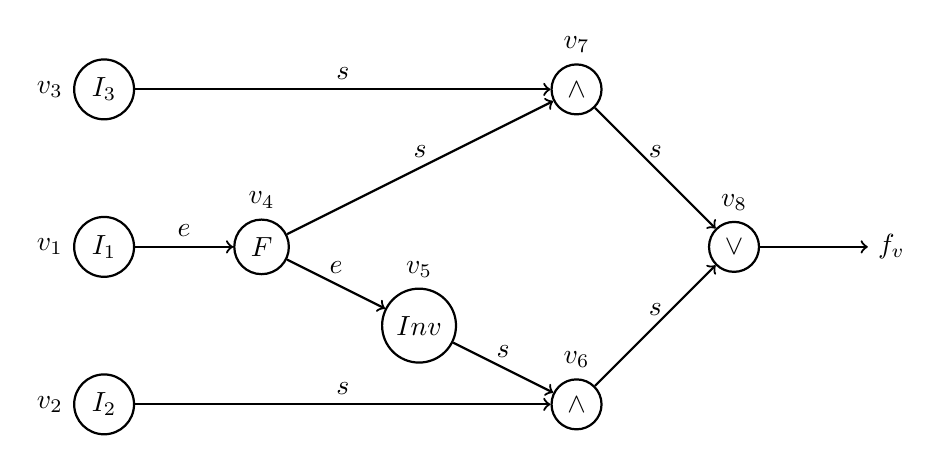
\begin{tikzpicture}[node distance={2cm and 2cm}, thick, scale=1, main/.style = {draw, circle}] 
	\node[main] (3) at (0,0) [label=west:$v_3$]{$I_3$}; 
	\node[main] (1) at (0,-2)[label=west:$v_1$] {$I_1$};
	\node[main] (2) at (0,-4)[label=west:$v_2$] {$I_2$};
	
	\node[main] (4) at (2,-2)[label=north:$v_4$]{$F$}; 
	
	\node[main] (5) at (4,-3)[label=north:$v_5$]{$Inv$};
	\node[main] (6) at (6,-4)[label=north:$v_6$]{$\wedge$};
	\node[main] (7) at (6,0)[label=north:$v_7$]{$\wedge$};
	
	\node[main] (8) at (8,-2)[label=north:$v_8$]{$\vee$};
	
	\node (f) at (10,-2) {$f_v$};
		
		
		\draw[->, above] (1) -- (4) node [midway] {$e$};
		\draw[->, above] (2) -- (6) node [midway] {$s$};
		\draw[->, above] (3) -- (7) node [midway] {$s$};
		\draw[->, above] (5) -- (6) node [midway] {$s$};
		\draw[->, above] (4) -- (5) node [midway] {$e$};
		\draw[->, above] (4) -- (7) node [midway] {$s$};
		\draw[->, above] (6) -- (8) node [midway] {$s$};
		\draw[->, above] (7) -- (8) node [midway] {$s$};
		\draw[->, above] (8) -- (f) node [midway] {};
		
		
	\end{tikzpicture}
	\caption{Logic Network of a 2:1 MUX with conditional coloring}\label{fig:mux_LN_clr}
\end{figure}

\subsection{New P\&R rule}

In this section, a new P\&R rule for conflicting gates in the ODN is proposed. The conflicting gates are the gates connected to PIs and colored $south$. The new rule is found to be effective not only inside the conflicting input area, but for the whole layout.

\begin{figure}
	\centering
	\subfigure[Placement rule of ortho]
	{
		\centering
		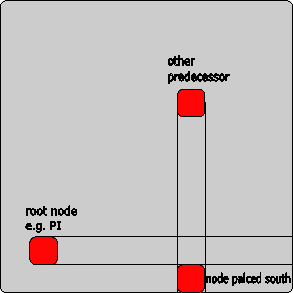
\includegraphics[scale=1.3]{south_scheme}
		\label{subfig:south_scheme}
	}
	\subfigure[Placement rule introduced with ODN]
	{
		\centering
		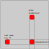
\includegraphics[scale=1.3]{new_south_scheme}
		\label{subfig:new_south_scheme}
	}
	\caption{Schematic representation of rules when placing nodes colored $south$}\label{fig:south_schemes}
\end{figure}

Looking at the original ortho algorithm part (lines 14-22) handling the placement of nodes based on their coloring makes sure that every gate placed $east$ occupies a new column and every node colored $south$ occupies a new row. These placement rules allow every gate to be placed without interfering with other gates, but the rules have been found to be too restrictive, allowing the following placement rule for $south$. Figure~\ref{fig:south_schemes} shows the $south$ rule of ortho and the $south$ rule introduced by the ODN. If a node is labeled $south$ and its predecessor, which has the lower horizontal position \textbf{also} has the higher vertical position, it is called \emph{root node} and the layout is \textbf{not} extended by a row while the gate is still in position $(w_p, h-1)$. Following this rule the gate is now placed in the same row as its root node and the same column as the predecessor with the higher x-coordinate. If we apply this to a two-input gate in the ODN with a PI and a fan-out node as predecessors, the PI is always the root node due to the ordering and new coloring. Thus, the new rule allows the two-input gate connected to the PI colored $south$ and the fan-out node to be placed in the same column as the PI, resulting in no conflict because the node is not \textit{actually} placed $south$ of its predecessors. It was found that this rule could not only be utilized for resolving PI conflicts, but also for the general $south$ placement in the algorithm with one exception. Though, considering a fan-out node to be the root node, the coloring would wire both the eastern and the southern colored outgoing edges onto the same row, yielding a conflict. For this case the new rule is not applied and this case is excluded for the input area through the ordering. The resulting pseudo-code snippets replacing the used code are shown in Algorithm~\ref{alg:input_network}.

Because this new rule can be applied not only for the input area but for all two-fan-in logic gates placed $south$ in the layout, area can be saved also for gates not viewed in the ODN.

\subsection{Inverter Balancing}

In this section a inverter balancing is introduced with the goal to reduce the number ove inverters in the logic network. Considering an inverter node is assigned $south$, such as after a fan-out node, and it is intended to be placed in the same row as a PI, a conflict arises because the input always has to wire in the x-direction. To minimize conflicts, all inverters colored $south$ must be placed at a minimum of one row further than the most southern PI.

To further reduce the number of inverters in the logic network and prevent excessive overhead and preserve all the advantages of the presented approach, an inverter balancing is introduced. This aims to reduce the number of inverters by substituting them at fan-out nodes. If a fan-out node has two inverters connected to its outgoing edges, these inverters can be replaced by a single inverter as the incoming node to the fan-out, resulting in an overall lower number of inverter nodes and preventing inverters in the ODN to be colored $south$.

Looking again at Figure~\ref{subfig:input_network_mux_21}, the placement and routing of the ortho algorithm after implementing the proposed ODN can be seen. The ordering of the inputs first places the fan-out node and then the two connected PIs. Since the inverter is part of the ODN it gets colored $east$ and allows the AND gates connected to the PIs to be colored $south$ and the new rule for placement and routing can be applied. The last OR gate is not part of the ODN and is therefore placed by the default rules of the ortho algorithm. In comparison to the layout in Figure~\ref{subfig:ortho_mux_21}, it can be quickly seen that the resulting layout saves up area and even wire crossings. The detailed results are presented and analyzed in the next chapter.

\begin{algorithm}[H]
	\vdots
	
	\begin{algorithmic}
		\State Convert $N$ to a 3-graph by substitution and balance inverters at fan-out nodes
		\State Order PI nodes
		\State \vdots
		\State Generate \textbf{conditional} direction assignment $d : \Delta \rightarrow \{east, south\}$ and subdivide signals if necessary
		\State Compute topological ordering $v_1, . . . , v_i \in N$
		\State Extend $L$ by one column and reserve it for PIs
		\ForAll {vertex $v_1, ..., v_i \in N $ with at most two incoming signals $\sigma_1, \sigma_2$}
		\If{vertex $v$ is terminal/PI}
		\State Extend $L$ by one row
		\State Place v at position $(0, h - 1)$
		\ElsIf{$d(\sigma_1) = d(\sigma_2) = east$}
		\State \vdots
		\ElsIf { signals are labeled $south$}
		\If{\textbf{not} root node exists}
		\State Extend $L$ by one row
		\EndIf
		\State $w_p \leftarrow$ max. horizontal position of v's predecessors
		\State Place v at position $(w _p, h - 1)$
		\EndIf
		
		\EndFor
		\State \vdots \\
		\Return $L$
	\end{algorithmic}
	\caption{Ortho changes with the ODN}\label{alg:input_network}
\end{algorithm}

\section{Majority Gate Distribution Network (MGDN)}\label{sec:majgatedisnet}
This section addresses the placement and routing of majority gates in QCA circuits using the ortho algorithm. The use of majority gates is significant in QCA as they can implement the majority function using only one gate, unlike in CMOS circuits which require multiple gates, as defined in Definition~\ref{Def:majf}. However, this theoretical advantage can only be realized through efficient placement and routing. To this end, a majority gates DN (MGDN) for the orthogonal algorithm is proposed, allowing for the placement and routing of majority gates and enabling a comparison of design metrics between a layout of a logic network in the MIG representation and its corresponding logic network in the AIG representation.

\subsection{The proposed signal Distribution Network}

\begin{figure}
	\centering
	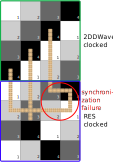
\includegraphics[scale=0.5]{Timing_failure_RES}
	\caption{Global sychronization violation when connecting 2DD-Wave and RES clocked scheme}\label{fig:Timing_failure_RES}
\end{figure}

The orthogonal algorithm uses 2DDWave clocking, which limits the direction assignment to only two options, $east$ and $south$, and can only handle the placement and routing of 2-input logic gates. To introduce "+"-majority gates into the layout, a RES-like clocking scheme is necessary, which includes tiles with three incoming tiles and one outgoing tile. As shown in Figure~\ref{subfig:RES}, such a tile is located at position $(1, 1)$ and is suitable for placing a "+" majority gate, allowing it to be connected with three incoming signals. However, changing the clocking scheme of ortho to RES would be highly inefficient and difficult to implement. This is because if the clocking scheme were completely changed to RES, the algorithm would not be able to utilize every row and column of the clocking. The RES scheme supports signals to flow into the western or northern directions, thus only the first and third rows and the second and fourth columns support eastern and southern signal propagation. This would lead to only these parts of the clocking being utilized for the placement of two-input gates, resulting in approximately double the area usage for only two-input logic gates.
An alternative approach to utilizing the RES scheme is to only support it in certain evenly distributed regions, allowing majority gates to be placed in specific, permanently assigned locations. For example, the layout could be divided into $4\times4$ tile sub-regions, and every fifth sub-region would be RES clocked, while the rest would be occupied with the 2DDWave scheme. On one hand, this approach should not produce as much area overhead since only some regions are inaccessible for two-input logic gates. However, the permanent clocking assignment limits the placement of majority gates to specific spots, leading to large area overhead if a majority gate needs to be placed far away from such a sub-region. For a network consisting mainly of majority gates, this implementation would also waste most of the 2DD-Wave clocked area. Another aspect to consider is the trivial global synchronization constraints within a uniformly 2DDWave clocked layout, which are disrupted by introducing RES clocking within the layout. By introducing irregular clocking such as RES sub-regions, signals can pass different amounts of tiles to reach the same tile, thereby violating the global synchronization constraint. In Figure~\ref{fig:Timing_failure_RES}, the top four rows are 2DD-Wave clocked and the bottom four rows are RES clocked. In the 2DD-Wave scheme, all three paths start globally synchronized. The two left paths need exactly one clock cycle to reach the majority gate. However, the right path in the RES scheme causes a delay, so that the signal travels two clock cycles before reaching the majority gate, thereby violating the global synchronization constraint.

%On the other hand, for the placement of three input majority gates a new direction assignment would have to be introduced to the logic network, since one signal would need a direction assignment $west$, changing the theory and complexity underlying the ortho algorithm.

\begin{figure}
	\centering
	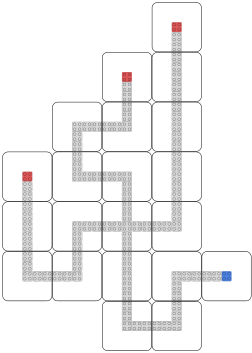
\includegraphics[scale=0.3]{Majority_Distribution_network}
	\caption{Proposed MGDN}\label{fig:QCA_Maj_nw}
\end{figure}


To overcome these complications, the proposed DN uses a custom clocking scheme only in areas where majority gates are placed, and addresses the global signal synchronization constraint. As a result, the placement and routing of solely two-input gates should not produce any additional area overhead. Figure~\ref{fig:QCA_Maj_nw} illustrates the proposed majority gate signal DN, which has been integrated into the ortho algorithm. The red marked cells indicate the three inputs for the MGDN. The cells in the middle of the tile are marked because they can be connected from above north or the west, which would result in one normal wire and one bent wire. The output marked blue allows the algorithm to wire it in the $east$ or $south$ direction, eliminating any limitations. It is also important to note that the input tiles as well as the output tiles have the same clocking number as in a regular 2DDWave scheme, allowing for seamless integration. Although the proposed DN does not produce any area overhead for the placement and routing of two-input gates, it can be seen that it does produce excess area for majority gates due to its complex wiring, resulting from the synchronization conditions that had to be considered in its design. In comparison to the implementation of an AIG representation of the majority function designed with the orthogonal algorithm, the placement and routing of this single majority gate already requires more area. However, it should be noted that no wire crossings are used. Assuming that wire crossings have a high cost, the proposed MGDN is considered less costly, although a meaningful cost comparison of the two implementations can only be done under a cost function that is informed by fabrication.

The design constraints used to develop the signal DN are discussed in the following. Firstly, the DN should not contain any wire-crossings as they are considered highly costly. Secondly, the DN must meet the global synchronization constraint. In a 2DDWave clocked layout, every diagonal is synchronous, and every signal wired on the same diagonal passes the same number of tiles following the orthogonal placement and routing. However, when examining the incoming tiles of a three-input tile, it can be seen that only two of the incoming tiles are on the same diagonal, meaning they are globally synchronized, and the third one is shifted by half a clock cycle. This results in the third incoming signal being delayed by half a clock cycle, violating the global synchronization constraint. Additionally, signals must pass a multiple of whole clock cycles in the signal DN in order to support the further use of 2DDWave and the local synchronization constraint. To satisfy this, the initially synchronous signals are first delayed by half a clock signal at the tile where the majority gate is placed, meeting the global synchronization constraint. Then, the output signal of the majority gate is delayed by another half a clock cycle, allowing it to be connected to the regular 2DDWave clocking scheme used in the remaining layout. The delays resulting from the DN lead to a total delay of one whole clock cycle for the signal propagating through the MGDN compared to all other signals in the logic network. Because the delay affects the global synchronization constraint, it has to be considered for each gate connected to the children of a MGDN. In the following, the basic placement and routing of the majority gates DN and the insertion of buffers in order to meet global synchronization is discussed.

\subsection{Placement and basic routing}

\begin{figure}
	\centering
	\begin{tikzpicture}[node distance={2cm and 2cm}, thick, main/.style = {draw, rectangle}] 
		\node[fit={(0,0) (8, 8)}, inner sep=0pt, draw=black, thick] (frame) {};
		\node[fit={(1,0) (7, 8)}, inner sep=0pt, draw=black, thick, fill=lightgray] (wires) {};
		\node[fit={(1,5) (3, 8)}, inner sep=0pt, draw=black, thick, fill=cyan] (logic) {C. logic \\ w/o MAJ};
		\node[fit={(3,4) (4, 5)}, inner sep=0pt, draw=black, thick, fill=yellow] (logic) {MAJ};
		\node[fit={(4,3) (5, 4)}, inner sep=0pt, draw=black, thick, fill=cyan] (logic) {};
		\node[fit={(5,2) (6, 3)}, inner sep=0pt, draw=black, thick, fill=yellow] (logic) {MAJ};
		\node[fit={(6,0) (7, 2)}, inner sep=0pt, draw=black, thick, fill=cyan] (logic) {};
		
		\node[fit={(0,6.5) (1, 8)}, inner sep=0pt, draw=black, thick, fill=TUMGray] (PIs) {PIs};
		\node[fit={(7,0) (8, 8)}, inner sep=0pt, draw=black, thick, fill=TUMGray] (POs) {POs};
		
		
		
		\draw (3.5,1) node [align = left] {Area for wiring \\ and buffer insertion};
		
		
	\end{tikzpicture} 
	\caption{Scheme of the P\&R using the MGDN} \label{fig:majority_scheme}
\end{figure}

The placement and routing of the proposed MGDN are subject to certain constraints. Firstly, the coloring of majority gates must be reviewed, as the logic network now includes three input nodes. However, the coloring algorithm can include auxiliary nodes to resolve coloring conflicts of edges, and therefore, by dividing every edge with a helping node, it can be seen that a trivial coloring can be found even when including three input nodes in the logic network. Another aspect to consider is the need for a new direction to connect a third signal to the majority gate. However, since the only time such wiring occurs is inside the fixed DN, which can be placed and routed in the usual south-eastern manner, no additional directions need to be included. Additionally, the irregular clocking inside the signal DN must be reviewed. These irregularities do not allow the algorithm to wire connections over the network, requiring a special treatment for the placement of the majority gates. From the algorithm's perspective, a majority gate cannot be placed just $south$ or $east$ of another gate, as these gates could need wiring through the MGDN. Instead, the algorithm is forced to always assign the MGDN to the $south$ and $east$ direction to prevent routing conflicts. This means that for majority gates, a naive coloring is always chosen. The major drawback of this is that the area is not used optimally and the layout is extended in two directions as shown in Figure~\ref{fig:majority_scheme}, compromising the beneficial use of the "+"-majority gate.

\subsection{Routing with signal synchronization and buffer insertion}
The placement and routing using the proposed DN results in a delay of one clock cycles of signals passing through a majority gate. Since the tile-based clocking does not support a speedup of a signal, every other signal which comes into contact with a delayed signal also has to be delayed in order to meet the global synchronization constraint. Therefore, a function is introduced to compute the delay of signals and allowing signals which are connected together to be synchronized by buffer insertion. For the delay computation, the algorithms views every incoming edge from every node starting at the PO. If an incoming edge is connected to a majority gate, every other incoming edge of the same node gets a delay of one assigned, if this edge is not also connected to a majority gate. In the latter, case all incoming edges of a node are delayed, resulting again in synchronous behavior. The inserted delays then result from the difference of delays of the incoming edges from a node and are realized by inserting wire buffers.

\begin{figure}
	\centering
	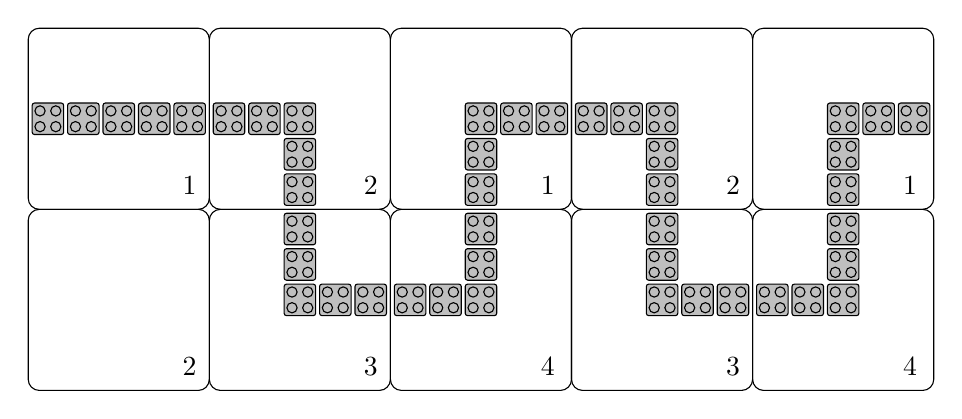
\begin{tikzpicture}
		\begin{scope}[xshift=-2.3cm, rotate=90]
			\draw[rounded corners] (-0.05, -0.1 - 0.85) rectangle (2.3-0.05, 2.3-0.1 - 0.85){};
			
			\foreach \x/\y in {0.9/0.9, 0.9/0.45, 0.9/0, 0.9/-0.45, 0.9/-0.9}
			{
				\draw[rounded corners = 0.3mm, fill=lightgray] (\x, 0 + \y) rectangle (1.2/3 + \x, 1.2/3 + \y){};
				\draw (0.3/3+ \x,0.3/3 + \y) circle (0.65mm);
				\draw (0.9/3+ \x,0.3/3+ \y) circle (0.65mm);
				\draw (0.3/3+ \x,0.9/3 + \y) circle (0.65mm);
				\draw (0.9/3+ \x,0.9/3 + \y) circle (0.65mm);
			}
			\node[text=black] (A1) at (0.25,-0.7) {$1$};
		\end{scope}
		\begin{scope}[xshift=-2.3cm, yshift=-2.3cm, rotate=90]
			\draw[rounded corners] (-0.05, -0.1 - 0.85) rectangle (2.3-0.05, 2.3-0.1 - 0.85){};
			
			\node[text=black] (A1) at (0.25,-0.7) {$2$};
		\end{scope}
		\begin{scope}[shift={(0, 0)}, rotate=90]
			\draw[rounded corners] (-0.05, -0.1 - 0.85) rectangle (2.3-0.05, 2.3-0.1 - 0.85){};
			
			\foreach \x/\y in {0.9/0.9, 0.9/0.45, 0.9/0, 0/0, 0.45/0}
			{
				\draw[rounded corners = 0.3mm, fill=lightgray] (\x, 0 + \y) rectangle (1.2/3 + \x, 1.2/3 + \y){};
				\draw (0.3/3+ \x,0.3/3 + \y) circle (0.65mm);
				\draw (0.9/3+ \x,0.3/3+ \y) circle (0.65mm);
				\draw (0.3/3+ \x,0.9/3 + \y) circle (0.65mm);
				\draw (0.9/3+ \x,0.9/3 + \y) circle (0.65mm);
			}
			\node[text=black] (A1) at (0.25,-0.7) {$2$};
		\end{scope}
		\begin{scope}[xshift=3.2cm, yshift=1.3cm, rotate=180]
			\draw[rounded corners] (-0.05, -0.1 - 0.85) rectangle (2.3-0.05, 2.3-0.1 - 0.85){};
			
			\foreach \x/\y in {0.9/0.9, 0.9/0.45, 0.9/0, 0/0, 0.45/0}
			{
				\draw[rounded corners = 0.3mm, fill=lightgray] (\x, 0 + \y) rectangle (1.2/3 + \x, 1.2/3 + \y){};
				\draw (0.3/3+ \x,0.3/3 + \y) circle (0.65mm);
				\draw (0.9/3+ \x,0.3/3+ \y) circle (0.65mm);
				\draw (0.3/3+ \x,0.9/3 + \y) circle (0.65mm);
				\draw (0.9/3+ \x,0.9/3 + \y) circle (0.65mm);
			}
			\node[text=black] (four) at (0.25 ,1.05) {$1$};
		\end{scope}
		\begin{scope}[xshift=-0.4cm, yshift=-0.1cm, rotate=270]
			\draw[rounded corners] (-0.05, -0.1 - 0.85) rectangle (2.3-0.05, 2.3-0.1 - 0.85){};
			
			\foreach \x/\y in {0.9/0.9, 0.9/0.45, 0.9/0, 0/0, 0.45/0}
			{
				\draw[rounded corners = 0.3mm, fill=lightgray] (\x, 0 + \y) rectangle (1.2/3 + \x, 1.2/3 + \y){};
				\draw (0.3/3+ \x,0.3/3 + \y) circle (0.65mm);
				\draw (0.9/3+ \x,0.3/3+ \y) circle (0.65mm);
				\draw (0.3/3+ \x,0.9/3 + \y) circle (0.65mm);
				\draw (0.9/3+ \x,0.9/3 + \y) circle (0.65mm);
			}
			\node[text=black] (A1) at (1.1+0.85,1.1) {$3$};
		\end{scope}
		\begin{scope}[xshift=1cm, yshift=-1.4cm, rotate=0]
			\draw[rounded corners] (-0.05, -0.1 - 0.85) rectangle (2.3-0.05, 2.3-0.1 - 0.85){};
			
			\foreach \x/\y in {0.9/0.9, 0.9/0.45, 0.9/0, 0/0, 0.45/0}
			{
				\draw[rounded corners = 0.3mm, fill=lightgray] (\x, 0 + \y) rectangle (1.2/3 + \x, 1.2/3 + \y){};
				\draw (0.3/3+ \x,0.3/3 + \y) circle (0.65mm);
				\draw (0.9/3+ \x,0.3/3+ \y) circle (0.65mm);
				\draw (0.3/3+ \x,0.9/3 + \y) circle (0.65mm);
				\draw (0.9/3+ \x,0.9/3 + \y) circle (0.65mm);
			}
			\node[text=black] (four) at (1.95 ,-0.65) {$4$};
		\end{scope}
		
		\begin{scope}[xshift=4.6cm, yshift=0cm, rotate=90]
			\draw[rounded corners] (-0.05, -0.1 - 0.85) rectangle (2.3-0.05, 2.3-0.1 - 0.85){};
			
			\foreach \x/\y in {0.9/0.9, 0.9/0.45, 0.9/0, 0/0, 0.45/0}
			{
				\draw[rounded corners = 0.3mm, fill=lightgray] (\x, 0 + \y) rectangle (1.2/3 + \x, 1.2/3 + \y){};
				\draw (0.3/3+ \x,0.3/3 + \y) circle (0.65mm);
				\draw (0.9/3+ \x,0.3/3+ \y) circle (0.65mm);
				\draw (0.3/3+ \x,0.9/3 + \y) circle (0.65mm);
				\draw (0.9/3+ \x,0.9/3 + \y) circle (0.65mm);
			}
			\node[text=black] (A1) at (0.25,-0.7) {$2$};
		\end{scope}
		\begin{scope}[xshift=7.8cm, yshift=1.3cm, rotate=180]
			\draw[rounded corners] (-0.05, -0.1 - 0.85) rectangle (2.3-0.05, 2.3-0.1 - 0.85){};
			
			\foreach \x/\y in {0.9/0.9, 0.9/0.45, 0.9/0, 0/0, 0.45/0}
			{
				\draw[rounded corners = 0.3mm, fill=lightgray] (\x, 0 + \y) rectangle (1.2/3 + \x, 1.2/3 + \y){};
				\draw (0.3/3+ \x,0.3/3 + \y) circle (0.65mm);
				\draw (0.9/3+ \x,0.3/3+ \y) circle (0.65mm);
				\draw (0.3/3+ \x,0.9/3 + \y) circle (0.65mm);
				\draw (0.9/3+ \x,0.9/3 + \y) circle (0.65mm);
			}
			\node[text=black] (four) at (0.25 ,1.05) {$1$};
		\end{scope}
		\begin{scope}[xshift=4.2cm, yshift=-0.1cm, rotate=270]
			\draw[rounded corners] (-0.05, -0.1 - 0.85) rectangle (2.3-0.05, 2.3-0.1 - 0.85){};
			
			\foreach \x/\y in {0.9/0.9, 0.9/0.45, 0.9/0, 0/0, 0.45/0}
			{
				\draw[rounded corners = 0.3mm, fill=lightgray] (\x, 0 + \y) rectangle (1.2/3 + \x, 1.2/3 + \y){};
				\draw (0.3/3+ \x,0.3/3 + \y) circle (0.65mm);
				\draw (0.9/3+ \x,0.3/3+ \y) circle (0.65mm);
				\draw (0.3/3+ \x,0.9/3 + \y) circle (0.65mm);
				\draw (0.9/3+ \x,0.9/3 + \y) circle (0.65mm);
			}
			\node[text=black] (A1) at (1.1+0.85,1.1) {$3$};
		\end{scope}
		\begin{scope}[xshift=5.6cm, yshift=-1.4cm, rotate=0]
			\draw[rounded corners] (-0.05, -0.1 - 0.85) rectangle (2.3-0.05, 2.3-0.1 - 0.85){};
			
			\foreach \x/\y in {0.9/0.9, 0.9/0.45, 0.9/0, 0/0, 0.45/0}
			{
				\draw[rounded corners = 0.3mm, fill=lightgray] (\x, 0 + \y) rectangle (1.2/3 + \x, 1.2/3 + \y){};
				\draw (0.3/3+ \x,0.3/3 + \y) circle (0.65mm);
				\draw (0.9/3+ \x,0.3/3+ \y) circle (0.65mm);
				\draw (0.3/3+ \x,0.9/3 + \y) circle (0.65mm);
				\draw (0.9/3+ \x,0.9/3 + \y) circle (0.65mm);
			}
			\node[text=black] (four) at (1.95 ,-0.65) {$4$};
		\end{scope}
		
	\end{tikzpicture}
	\caption{Buffer in $east$ direction with respective clocking}\label{fig:QCA_buf}
\end{figure}

Figure~\ref{fig:QCA_buf} depicts a buffer in the $east$ direction, which can also be used in the $south$ direction by just rotating it by $90$ degrees. The snake-shaped structure delays a signal by exactly one clock cycle, but can be extended for any number of clock cycles. This structure is also used in custom placement and routing resulting from the QCA ONE library~\cite{QCA_scl}. As in the MGDN, the buffers support irregular clocking, creating zones through which the algorithm cannot wire. In the case of buffers only one column or row is made impassable, introducing a rewiring for conflicts. Algorithm~\ref{alg:majority_network} shows the code snippets which are changed and added to ortho in order to allow the placement and routing of MGDNs. Figure~\ref{fig:majority_with_buf} shows the placement of a majority gate inside the input DN and one AND gate that needs the incoming signal from the PI to be delayed in order to match the delay of the connected MGDN. The insertion of the buffer happens in $south$ direction, while one column is held free in order to resolve any upcoming conflict. From this layout, it can already be seen that the implementation of the MGDN brings several complications with it, all resulting in area overhead, which stands in contrast to the area which should be saved by introducing majority gates in the first place.

\begin{algorithm}[H]
	\vdots
	
	\begin{algorithmic}
		\State Convert $N$ to a 3-graph by substitution and balance inverters at fan-out nodes, except for majority gates
		\State Compute the delay as majority buffer insertion $buf_{maj}$ for every node and assign it to the incoming signals $\sigma$
		\State Order PI nodes
		\State Create vectors with from the majority buffers blocked columns $bl_c$ and rows $bl_r$
		\State \vdots
		\ForAll {vertex $v_1, ..., v_i \in N $ with at most three incoming signals $\sigma_1, \sigma_2, \sigma_3$}
		\State Rewire incoming signals which are wired on $bl_c$ or $bl_r$
		\State \vdots
		\If{vertex $v$ has fanin of three (is a majority gate)}
		\If{$d(\sigma_1) = d(\sigma_2) = d(\sigma_3) = south$}
		\State{Extend $L$ by one row and wire the incoming signal to $(w_p, h-1)$ for every incoming signal}
		\EndIf
		\State Insert majority buffers according to the delay computed in $buf_{maj}$ and safe blocked columns $bl_c$ and rows $bl_r$
		\State Extend the layout by number of rows $(7)$ and columns $(5)$ of the MGDN and place the DN at $(w-5, h-7)$
		\State Connect incoming signals west to the inputs of the DN
		\ElsIf{$d(\sigma_1) = d(\sigma_2) = east$}
		\State Insert majority buffers according to the delay computed in $buf_{maj}$ and safe blocked rows $bl_r$
		\State \vdots
		\ElsIf { signals are labeled $south$}
		\State Insert majority buffers according to the delay computed in $buf_{maj}$ and safe blocked columns $bl_c$
		\State \vdots
		\EndIf
		
		\EndFor
%		\State \vdots \\
%		\Return $L$
	\end{algorithmic}
	\caption{Ortho changes with MGDN}\label{alg:majority_network}
\end{algorithm}

\begin{figure}
	\centering
	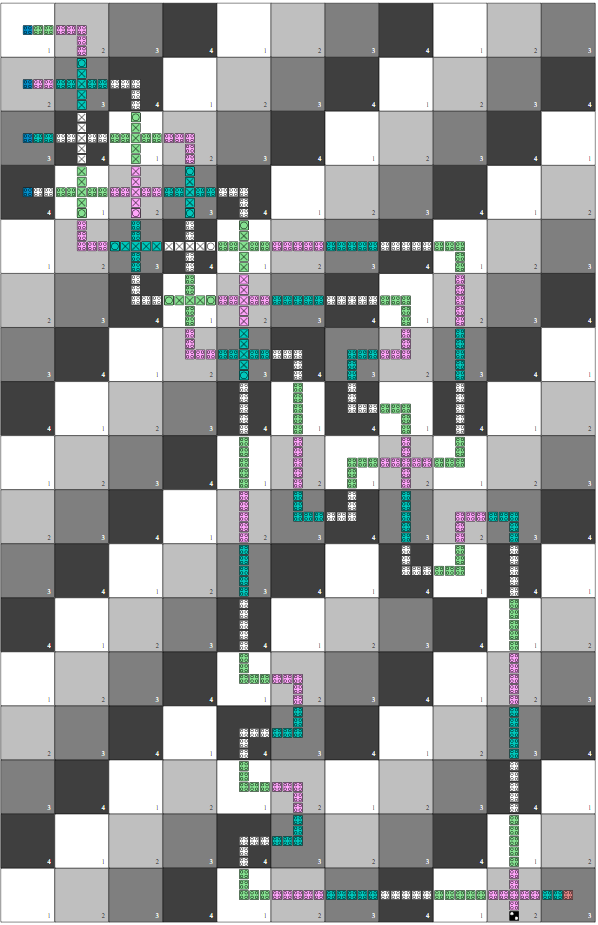
\includegraphics[scale=0.65]{maj_example}
	\caption{Placement and routing of a majority gate in conjunction with a delayed PI}\label{fig:majority_with_buf}
\end{figure}


\section{Sequential Distribution Network (SDN)}
In this section, a DN that enables ortho automatic design of sequential circuits is presented. To the authors' knowledge, there is currently no solution for automatically placing and routing sequential circuits in QCA. The existing algorithms for handling sequentiality in QCA, discussed in Chapter~\ref{chapter:SotA}, simply translate CMOS structures into QCA and rely on an additional external clock signal, which is considered unnatural in the context of QCA's inherent clocking paradigm. The proposed placement and routing method utilizes the concept of signal-delaying wires from~\cite{Walter}, and builds upon it to enable automatic placement and routing.

\subsection{Placement and Routing}
Before delving into the algorithm, it is important to first discuss the concept of a FF wire in the context of placement and routing, rather than just considering it as a standalone element. The proposed FF implementation in QCA requires more complex clock generators for each FF, and it is uncertain if this is possible to implement. From the basic architecture of sequential circuits, we can see that a sequential circuit includes a combinational logic block and a storage element, which is formed by a FF wire in QCA. However, in contrast to CMOS, where the information can be arbitrarily wired back from the storage to the inputs of the combinational logic, in QCA, wiring back implies the placement of wire segments, each of which delays the information by one clocking zone, acting as a partial FF. When a signal is wired through four adjacent wire gates, a basic FF is formed, since the information is delayed by four clock zones, equivalent to one clock cycle. This delay is the purpose of a clocking element, and the reason why the clocking for the wire FF is customized. The proposed idea in this work is to use the natural delay that occurs due to sequential wiring to mimic storage elements, reducing the need for customized clocking and allowing wire segments to be summarized as FFs.

\begin{figure}
	\centering
	\begin{tikzpicture}[node distance={2cm and 2cm}, thick, main/.style = {draw, rectangle}] 
		\node[fit={(0,0) (8, 8)}, inner sep=0pt, draw=black, thick] (frame) {};
		\node[fit={(2,2) (6, 8)}, inner sep=0pt, draw=black, thick, fill=cyan] (logic) {Combinational logic};
		\node[fit={(0,6.5) (1, 8)}, inner sep=0pt, draw=black, thick, fill=TUMGray] (PIs) {PIs};
		\node[pattern=north west lines, pattern color=TUMGray, fit={(1,6.5) (2, 8)}, inner sep=0pt, draw=black, thick] (wires) {wires};
		\node[fit={(1,5) (2, 6.5)}, inner sep=0pt, draw=black, thick, fill=lightgray] (ROs) {ROs};
		\node[pattern=north west lines, pattern color=TUMGray,fit={(6,3.5) (7, 8)}, inner sep=0pt, draw=black, thick] (wires) {wires};
		\node[fit={(7,3.5) (8, 8)}, inner sep=0pt, draw=black, thick, fill=TUMGray] (POs) {POs};
		\node[fit={(6,2) (7, 3.5)}, inner sep=0pt, draw=black, thick, fill=lightgray] (RIs) {RIs};
		
		\draw[] (7, 3.5) -- (8, 3.5);
		\draw[] (0, 6.5) -- (1, 6.5);
		\draw[fill=Apricot] (0, 0) -- (0, 6.5) -- (1, 6.5)  -- (1, 5) -- (2, 5) -- (2, 2) -- (7, 2) -- (7, 3.5) -- (8, 3.5) -- (8, 0) -- (0, 0);
		\draw (4,1) node [align=left] {Sequential wires from Ris to Ros \\ with delay of $c$ clock cycles};
		%		\draw[->] (2) -- (5);
		%		\draw[->] (3) -- (6);
		%		\draw[->] (4) -- (6);
		%		\draw[->] (5) -- (7);
		%		\draw[->] (6) -- (7);
		%		\draw[->] (7) -- (f);
		
	\end{tikzpicture} 
	\caption{Scheme of a sequential circuit layout after placement and routing} \label{fig:sequential_gate_sample}
\end{figure}

Considering the placement and routing of sequential circuits, not only a DN has to be designed but also the logic network has to be expanded regarding to storage elements. They are represented in the logic network by registers with its corresponding input, determining the value, which has to be stored, and its output, which gives the register value to the combinational logic again after delaying it to the next \textit{circuit clocking cycle}. A circuit clocking cycle refers to one cycle of Bennett clocking that has propagated through the circuit completely. The registers are implemented into the logic network as follows. Register inputs (RIs) are treated similar to POs, therefore they are dangling edges, which point to no node but additionally have a RO (RO) assigned. ROs are treated similarly to PIs, being terminal vertices, but always feeding in the data which were given to the corresponding RI in the last circuit clocking cycle. Therefore, the logic network extends to $N = (\Lambda, I, RO, \Sigma, O, RI)$. Here it has to be mentioned that for the input DN due to their similarity ROs can be treated just like PIs, enabling the combination with the SDN.

Also, for placement and routing, the similarities between PIs/ROs and POs/RIs can be exploited. The schematic layout resulting from the described algorithm is shown in Figure~\ref{fig:sequential_gate_sample}. When the first part of ortho is performed, first the combinational logic part is placed and routed, treating ROs like PIs and RIs like POs, wiht the only difference, that PIs and PO are wired to the borders. From this stage, a routing from the RIs to the ROs has to be found, which retains the local and global synchronization constraint. Because every RI has exactly one RO assigned, first of all, the RIs are rewired and sorted in the same order as the ROs. The ordering follows in a way that all RIs are put on a diagonal, and since to this point every gate is clocked uniformly with 2DDWave, the signals are all synchronized. With this starting position, now wires with the same length have to be found between every RI and output. Since the wires now also have to go in western and northern directions in order to close the loop between the ROs in the upper left corner and the RIs in the down-right corner of the layout, the wiring is not arbitrary. Another big issue is that the clocking cannot be chosen independently for each back-loop because the loops cross each other. Also the global timing constraint has to be viewed again. Considering a PI in a completely combinational circuit being placed in the fifth row of the layout. In this case the PI is set in a different \textit{time zone}, because its signal is globally delayed by one clock cycle. Until now the assumption was made, that an input network can be used to delay the PI by one clocking cycle to achieve again global synchronization. When an RO is placed in a different time zone, this also has to be respected by the wiring of the registers. As already mentioned, the registers do not delay the information by only one clocking cycle but by multiple clocking slowing down the performance of the circuit drastically. This huge delay is due to the fact that ortho lays the combinational logic only in the south-eastern direction, always increasing the distance between PIs/ROs and POs/RIs. Therefore the sequential signal DN always grows with the size of the combinational logic.

For further research, maybe a folding operation can be found for the ortho algorithm so that the distance between RIs and ROs can be decreased, and therefore, the delay produced by the SDN can be decreased as well.

\begin{algorithm}[H]
	\vdots
	
	\begin{algorithmic}
		\If{vertex $v$ is PI}
		{
			\State Extend $L$ by one row
			\State Place v at position $(0, h - 1)$
			\State Wire the PI to position $(num_{reg}*2, h - 1)$ 
			\If{vertex $v$ is colored $south$}
			\State Extend $L$ by one column
			\State Wire the PI to position $(w - 1, h - 1)$ 
			\EndIf
		}
		\ElsIf{vertex $v$ is RO}
		{
			\State Extend $L$ by one row
			\State Place v at position $(num_{reg}*2, h - 1)$
			\If{vertex $v$ is colored $south$}
			\State Extend $L$ by one column
			\State Wire the PI to position $(w - 1, h - 1)$ 
			\EndIf
		}
		\State\vdots
		\EndIf
		\State Connect the primary outputs to the respective borders
		\State Connect the RIs to the respective borders and connect the RIs to the ROs
		\Return $L$
		
		
	\end{algorithmic}
	\caption{Ortho changes with SDN}\label{alg:seq_network}
\end{algorithm}

\subsection{RAM cell}
As previously discussed in Section~\ref{subsec:RAM_SoA}, a RAM cell can be implemented using wire delays to temporarily store data. Figure~\ref{fig:QCA_RAM} illustrates a RAM cell, including its WL, BL, and register components. The cell comprises of two main components: a 2:1 MUX and a register. The register transfers data from the output to one of the inputs of the MUX, which then determines whether new data should be written to the cell or if the existing data should be retained. It is worth noting that the depicted RAM cell was designed manually, however, the proposed SDN is also able to layout a RAM cell, but with the drawback of increased layout area and slower operation.

\begin{figure}
	\centering
	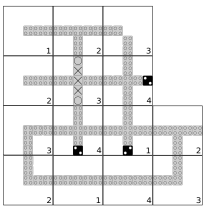
\includegraphics[scale=0.4]{MUX_RAM}
	
%	\subfigure[Truth table]
%	{
%		% Table generated by Excel2LaTeX from sheet 'Tabelle1'
%		\centering
%		\begin{tabular}{cllll}
%			& Input1 & Input2 & Input3 & Output \\
%			\multirow{2}[0]{*}{Maj1} & $WL_1$   & $WL_2=\overline{WL_1}$ & $BL$    & $BL$ \\
%			& $WL_1=\overline{BL}$ & $WL_2=\overline{BL}$ & $BL$    & $\overline{BL}$ \\
%			\multirow{2}[0]{*}{Maj2} & $X$     & $BL$    & $BL$    & $BL$ \\
%			& $X$     & $\overline{BL}$ & $BL$    & $X$ \\
%		\end{tabular}%
%		\label{subfig:QCA_RAM_tt}
%	}
	\caption{QCA RAM cell designed as 2:1 mux with a SDN}\label{fig:QCA_RAM}
\end{figure}